\section{MNIST Dataset} \label{sec:prob4}
In this section, we use each of the algorithms to classify handwritten digits from the MNIST dataset.

\subsection{Part 1}
The MNIST dataset contains labeled, handwritten digits.
We split the dataset into multiple classification tasks, shown in the first column of~\cref{table_4_1}.
We also split it into training, validation, and testing sets.

We follow the typical procedure: train with many hyperparameters (C for $L_1$, $L_2$ for LR, and C for SVM), choose the hyperparameters that maximize performance on the validation set with lowest model complexity (low C), and report performance on the test set for the best hyperparameters.

The two classifiers here, Logistic Regression and Linear SVM, perform similarly on each classification task.
For all tasks, the training accuracy was better than the testing accuracy, as expected.

Normalization of the data did not make a large difference ($<\pm 1\%$) for these classifiers, and results presented are for non-normalized data.
The only significant difference after normalization was the size of regularization constant $C$; in all cases, normalization caused the optimal $C$ value to increase by a few orders of magnitude.
This is likely because the size of the data elements decreased, so the size of the learned weight vector increased, meaning a smaller regularization cost had to be applied for the same effect.

A couple misclassified digits are shown in~\cref{fig:misclassified}.
Some handwriting is very difficult even for humans to classify, so it makes sense that our learned classifiers are not perfect.

\begin{figure}\label{fig:misclassified}
    \centering
    \begin{subfigure}[b]{0.5\columnwidth}
        \centering
        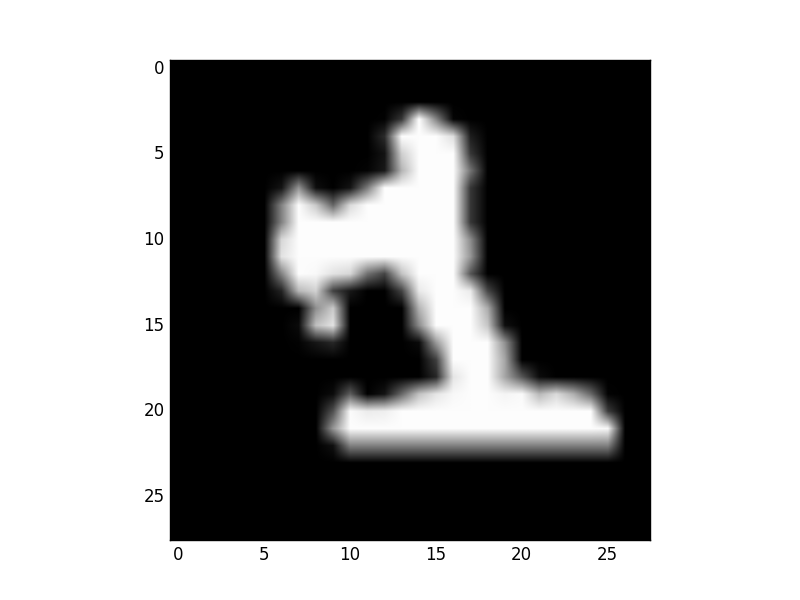
\includegraphics[height=1.2in]{figures/4_1_bad1}
        \caption{Misclassified 1}
    \end{subfigure}%
    ~ 
    \begin{subfigure}[b]{0.5\columnwidth}
        \centering
        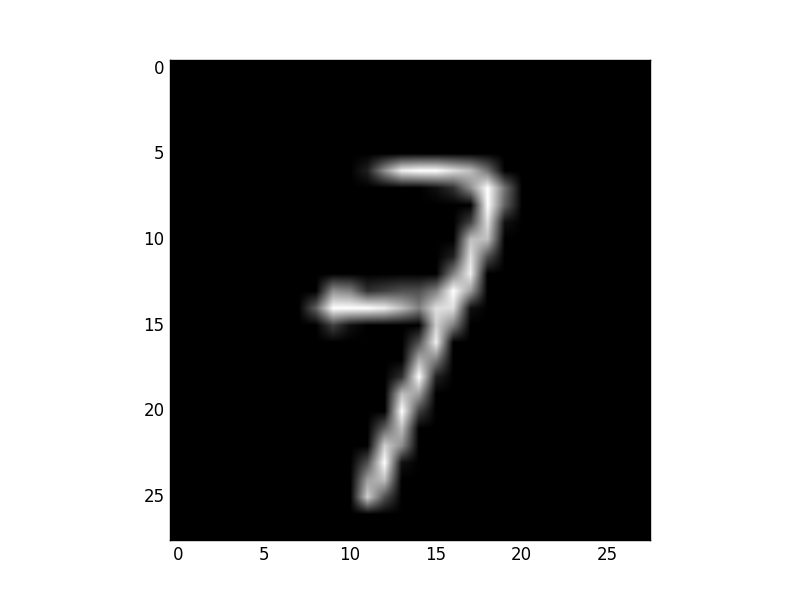
\includegraphics[height=1.2in]{figures/4_1_bad7}
        \caption{Misclassified 7}
    \end{subfigure}
    \caption{The MNIST dataset has some ambiguous entries, in accordance with real human handwriting, that are difficult to classify correctly.}
\end{figure}

\begin{table}[ht!]
\centering
\begin{tabular}{||c c c c c||}  
 \hline
 Dataset & LR Tr. & LR Test & SVM Tr & SVM Test \\ [0.3ex] 
 \hline\hline
 1 vs. 7 & 100.0 & 98.3 ($C=1$) & 100.0 & 98.7 ($C=0.2$) \\ 
 \hline
 3 vs. 5 & 100.0 & 93.3 ($C=60$) & 100.0 & 94.7 ($C=0.02$) \\ 
 \hline
 4 vs. 9 & 100.0 & 94.7 ($C=2$) & 100.0 & 94.7 ($C=0.02$) \\ 
 \hline
 odds vs. evens & 92.9 & 89.0 ($C=0.1$) & 93.9 & 89.2 ($C=0.02$) \\ 
 \hline
\end{tabular}
\caption{Accuracy of LR and Linear SVM on MNIST datasets.}
\label{table_4_1}
\end{table}

\subsection{Part 2}
Next, we applied the Gaussian RBF SVM classifier on the MNIST dataset for the same binary classification tasks.
Again, there are two parameters, $C$ (regularization) and $\gamma$ (bandwidth) that must be tuned with the validation set.
It is difficult to tune these two in parallel, especially without a method of visualizing the dataset, as was possible in the simple 2D data case.
Our approach was to train of each parameter in the range $[10^{-5}, 10^{-4}, ..., 10^{5}]$, and then compare accuracy on the validation set.
Many models had a validation accuracy of 100\%, so for these, the least complex model (low $\gamma$, low $C$).
The choice of $C$, $\gamma$, and training and test accuracy are shown in~\cref{table_4_2}.
Even with the worst choice of parameters in the stated range, validation accuracy was around 70-80\%, so the classifier was not completely useless.
For each classification task, the hyperparameters $C=10^{-5}$, $\lambda=0.1$ were chosen.


[todo: compare rbf to linear classifiers]

[todo: finish table]

\begin{table}[ht!]
\centering
\begin{tabular}{||c c c||}  
 \hline
 Dataset & Tr. Acc & Test Acc \\ [0.3ex] 
 \hline\hline
 1 vs. 7 & 100.0 & 98.3 \\ 
 \hline
 3 vs. 5 & 100.0 & 93.3 \\ 
 \hline
 4 vs. 9 & 100.0 & 94.7 \\ 
 \hline
 odds vs. evens & 100.0 & 76.1 \\ 
 \hline
\end{tabular}
\caption{Accuracy of Gaussian RBF SVM classifier on MNIST datasets.}
\label{table_4_2}
\end{table}

\subsection{Part 3}
[todo]

